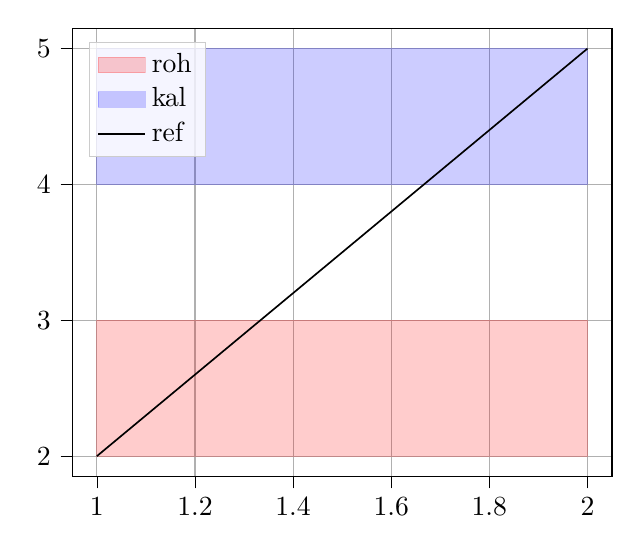
\begin{tikzpicture}

\definecolor{darkgray176}{RGB}{176,176,176}
\definecolor{lightgray204}{RGB}{204,204,204}

\begin{axis}[
legend cell align={left},
legend style={
  fill opacity=0.8,
  draw opacity=1,
  text opacity=1,
  at={(0.03,0.97)},
  anchor=north west,
  draw=lightgray204
},
tick align=outside,
tick pos=left,
x grid style={darkgray176},
xmajorgrids,
xmin=0.95, xmax=2.05,
xtick style={color=black},
y grid style={darkgray176},
ymajorgrids,
ymin=1.85, ymax=5.15,
ytick style={color=black}
]
\path [draw=red, fill=red, opacity=0.2]
(axis cs:1,3)
--(axis cs:1,2)
--(axis cs:2,2)
--(axis cs:2,3)
--(axis cs:2,3)
--(axis cs:1,3)
--cycle;
\addlegendimage{area legend, draw=red, fill=red, opacity=0.2}
\addlegendentry{roh}

\path [draw=blue, fill=blue, opacity=0.2]
(axis cs:1,5)
--(axis cs:1,4)
--(axis cs:2,4)
--(axis cs:2,5)
--(axis cs:2,5)
--(axis cs:1,5)
--cycle;
\addlegendimage{area legend, draw=blue, fill=blue, opacity=0.2}
\addlegendentry{kal}

\addplot [semithick, black]
table {%
1 2
2 5
};
\addlegendentry{ref}
\end{axis}

\end{tikzpicture}
